\begin{figure}[htbp]
\centering
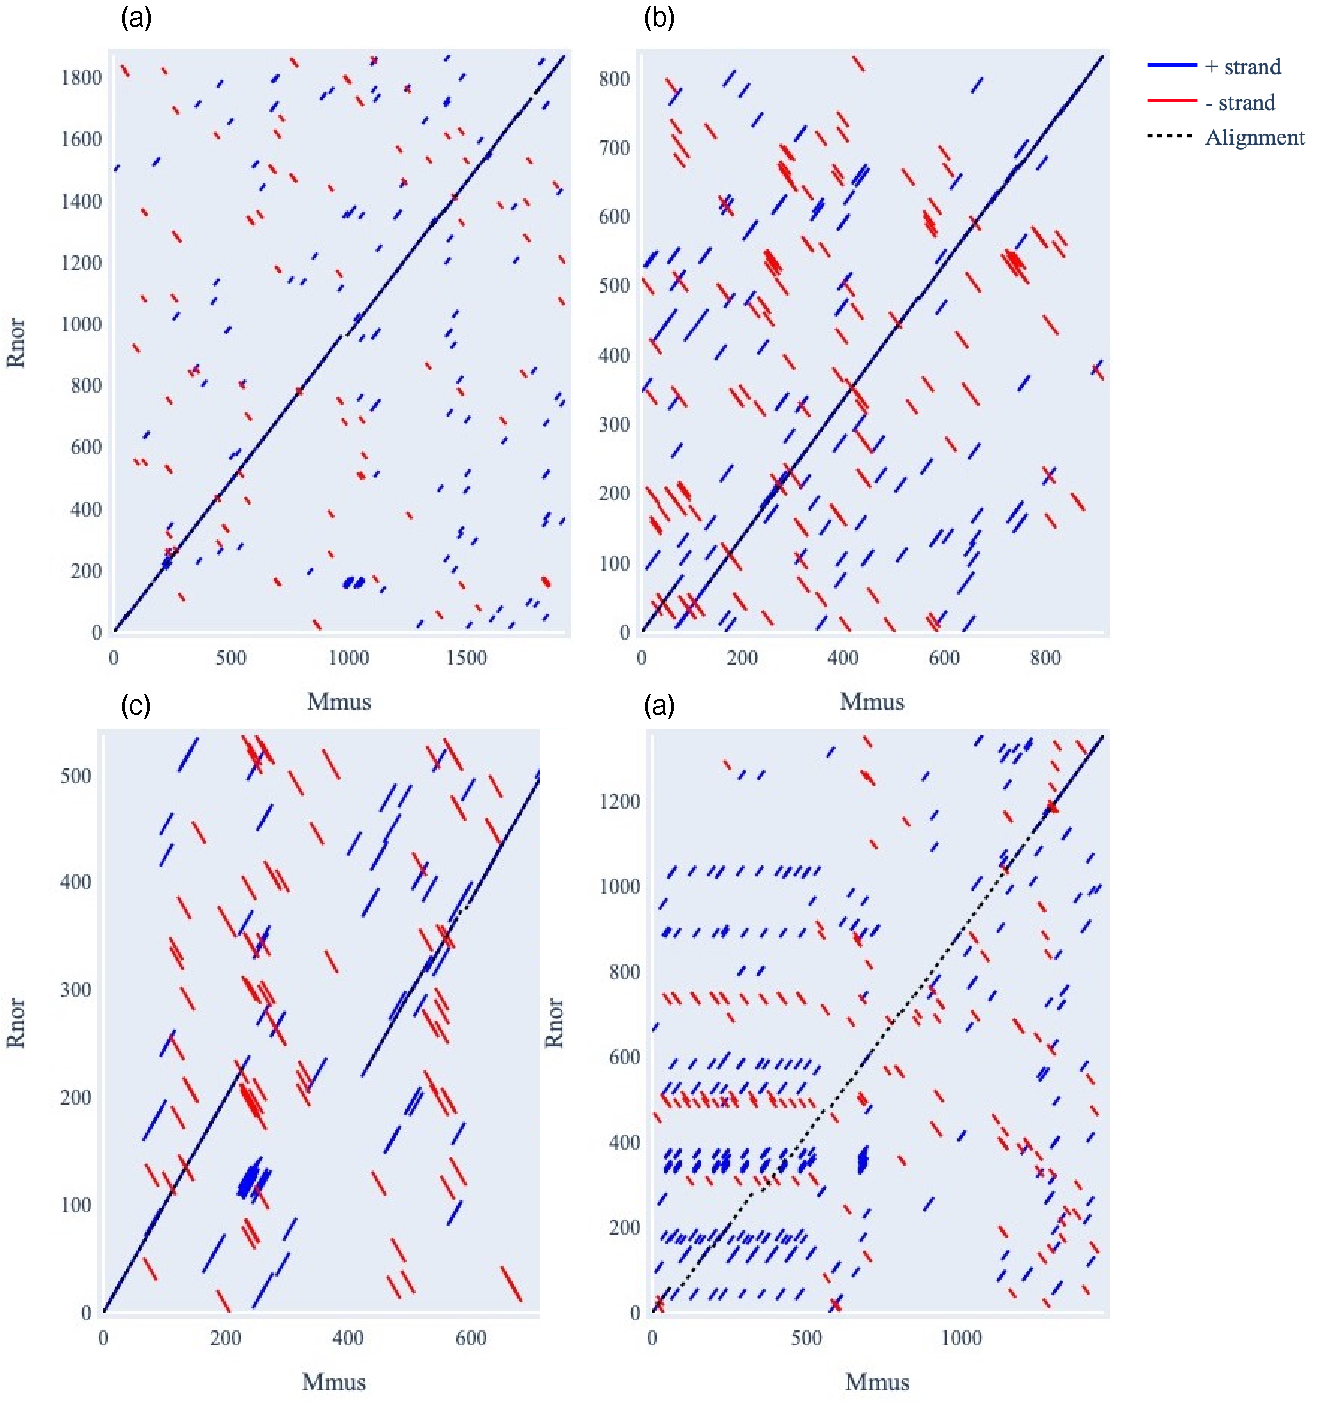
\includegraphics[width=\textwidth]{figures/diagrams/fxy_dotplot_2.pdf}
\caption[Dotplots of \textit{Fxy} introns 5-8]{ \textbf{Dotplots of \textit{Fxy} introns 5-8}.  The alignment path between the sequences is shown as the dotted line. Long stretches of identity between sequences form a diagonal. The window was 20bp long, 20-mers identical at $>13$ positions were considered a match. The $x$- and $y$-axis are positions in the unaligned sequence. Introns 7 and 8 were excluded from analyses due to their  visually poor alignment paths, subplot (c) and (d) respectively. }
\label{fig:Fxy-dp-2}
\end{figure}